\chapter{Study Gap}

\section{Research Gap}

\section{Objectives}

\paragraph{Filler Text} \lipsum[1]
%
\begin{figure}[t]
  \centering
  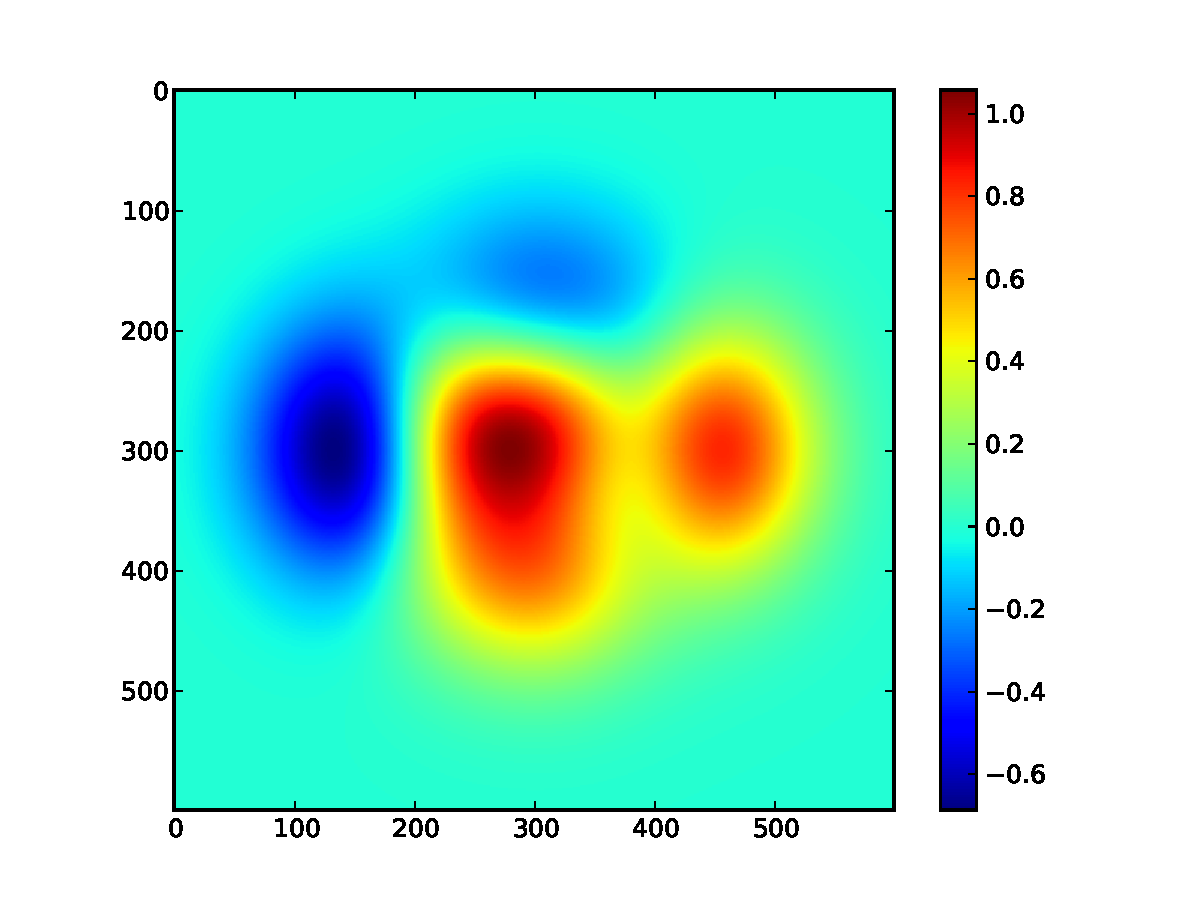
\includegraphics[width=0.6\textwidth]{Chapter-2/figs/color}
  \caption{A figure at the top of the page.}
  \label{fig:ch3.1}
\end{figure}
%
\lipsum[2]
%
\begin{figure}[!h]
  \centering
  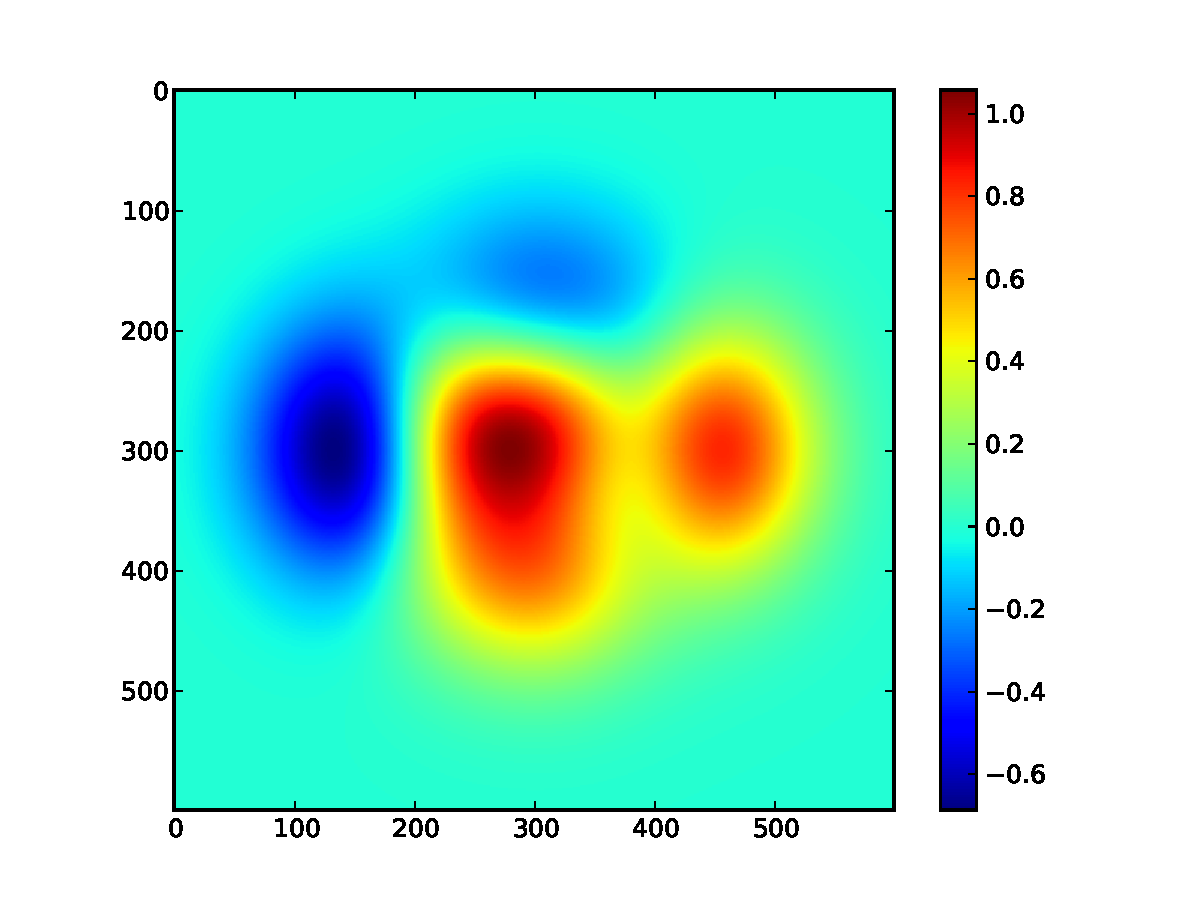
\includegraphics[width=0.6\textwidth]{Chapter-2/figs/color}
  \caption{A figure in the middle of text.}
  \label{fig:ch3.2}
\end{figure}
%
\begin{figure}[!b]
  \centering
  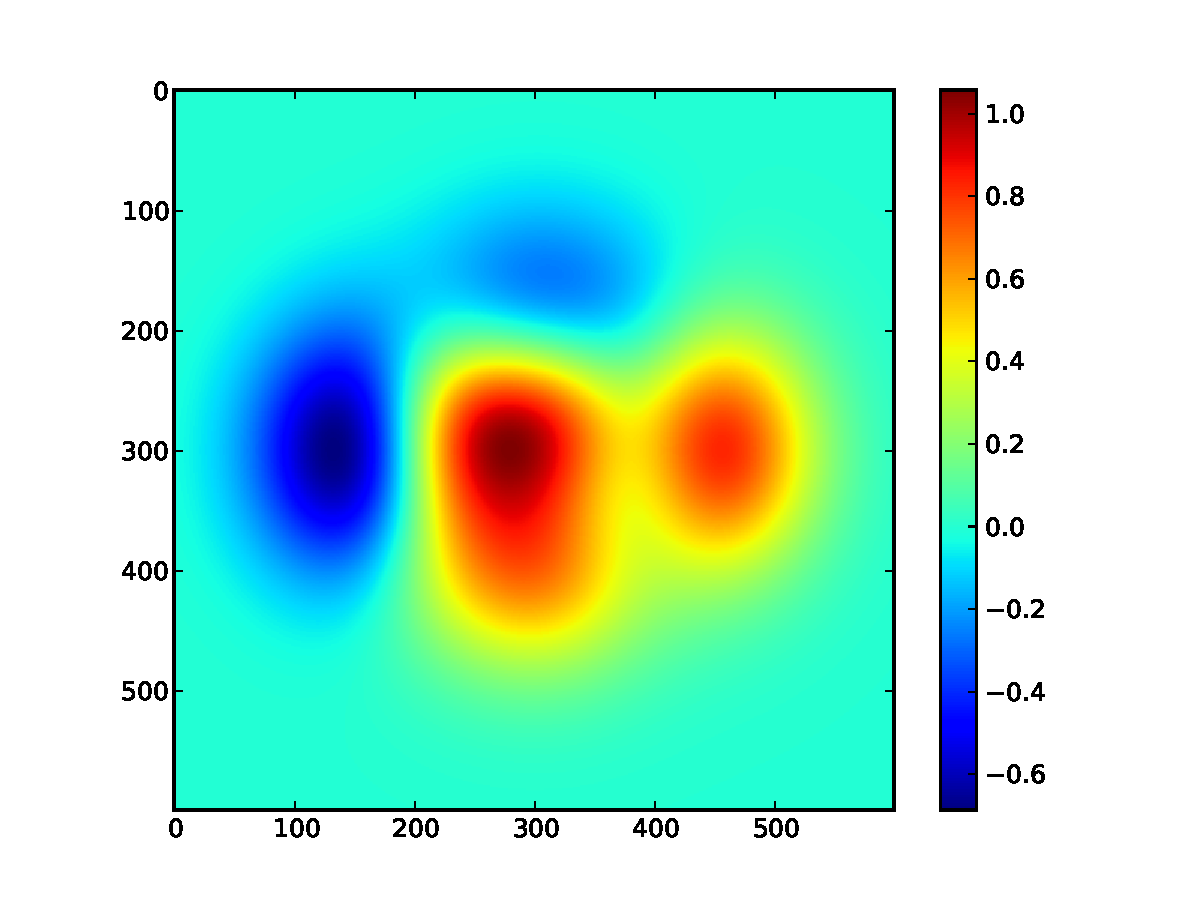
\includegraphics[width=0.6\textwidth]{Chapter-2/figs/color}
  \caption{A figure at the bottom of the page.}
  \label{fig:ch3.3}
\end{figure}
%
\lipsum[3]
